%%%%%%%%%%%%%%%%%%%% chapter.tex %%%%%%%%%%%%%%%%%%%%%%%%%%%%%%%%%%
% Chapter 7: Thermal Modeling, Hotspots & Fault-Tolerant Resilience
% Springer Nature Monograph svmono format
%%%%%%%%%%%%%%%%%%%%%%%%%%%%%%%%%%%%%%%%%%%%%%%%%%%%%%%%%%%%%%%%%%%

\chapter{Thermal Modeling, Hotspots \& Fault-Tolerant Resilience}
\label{chap:thermal-faults}

\abstract*{As semiconductor manufacturing scales into deep sub-micron nodes, thermal power density has emerged as a fundamental roadblock limiting multi-core performance. In high-performance Networks-on-Chip (NoC), non-uniform traffic patterns concentrate dynamic switching activity within localized routers, producing extreme thermal hotspots that accelerate electromigration and trigger catastrophic sub-threshold leakage runaway. This chapter provides a comprehensive treatment of interconnect thermal physics and silicon resilience. We first formalize the compact electro-thermal RC duality established by the HotSpot methodology, deriving the continuous and discrete state-space governing equations for multi-core heat conduction. Next, we address the challenge of on-chip thermal telemetry under non-Gaussian sensor noise, analyzing the Gaussian-Sum Filter (GSF) architecture and Huber M-estimation developed by Fu et al. (IEEE TCAD 2019). We then examine proactive hotspot prediction using hardware-synthesizable Artificial Neural Networks (ANNs) based on Kakoulli et al. (IEEE TCAD 2012), demonstrating how predictive traffic throttling mitigates hotspot emergence hundreds of cycles before buffer saturation occurs. Finally, we explore silicon fault tolerance in 2D meshes without virtual channels, presenting the ZoneDefense framework (Fu et al., IEEE TVLSI 2014) for convex fault block containment and defense zone detour routing, accompanied by synthesizable Verilog router bypass logic and cycle-accurate thermal simulation models.}

\section{The Thermal Emergency in Deep Sub-Micron Silicon}
\label{sec:thermal-emergency}

In modern sub-5\,nm multi-core architectures, power density frequently exceeds $100\,\mathrm{W/cm^2}$---a thermal flux comparable to the surface of the sun. Networks-on-Chip (NoC) routers and high-speed serial links contribute between $20\%$ to $40\%$ of overall chip power dissipation. Because network traffic is intrinsically bursty and spatially non-uniform, switching activity concentrates at topological bottlenecks (such as memory controller interfaces and bisection crossbars), forming extreme localized temperature spikes termed \emph{thermal hotspots}.

The physical consequences of unmitigated thermal hotspots are severe across three fundamental dimensions:
\begin{enumerate}
    \item \textbf{Sub-Threshold Leakage Runaway}: Sub-threshold leakage current exhibits an exponential dependence on absolute operating temperature governed by the Arrhenius formulation:
    \begin{equation}
        I_{\mathrm{leak}}(T) \propto T^2 \exp\left(-\frac{q V_{\mathrm{th}}}{m k_B T}\right)
        \label{eq:arrhenius-leakage}
    \end{equation}
    where $V_{\mathrm{th}}$ is the threshold voltage, $k_B$ is Boltzmann's constant, and $q$ is the elementary electron charge. As local silicon heats up, $V_{\mathrm{th}}$ drops while thermal carrier excitation intensifies, triggering a positive feedback loop that culminates in \emph{thermal runaway}.
    
    \item \textbf{Carrier Mobility Degradation}: Acoustic phonon scattering increases with temperature, degrading electron and hole mobility according to:
    \begin{equation}
        \mu(T) = \mu(T_0) \left(\frac{T}{T_0}\right)^{-1.5}
        \label{eq:mobility-degradation}
    \end{equation}
    Reduced mobility diminishes transistor drive current ($I_{\mathrm{on}}$), expanding router pipeline gate delays and causing timing closure violations.
    
    \item \textbf{Accelerated Electromigration}: Spatial thermal gradients across adjacent router tiles induce intense thermo-mechanical shear stress due to mismatched coefficients of thermal expansion (CTE). Furthermore, according to \emph{Black's Equation}, the Mean Time to Failure ($MTTF$) of copper interconnects drops exponentially with temperature:
    \begin{equation}
        MTTF = \frac{A}{J^n} \exp\left(\frac{E_a}{k_B T}\right)
        \label{eq:blacks-equation}
    \end{equation}
    where $J$ is the current density and $E_a \approx 0.9\,\mathrm{eV}$ is the activation energy for copper grain-boundary diffusion. A temperature increase of only $15^\circ\mathrm{C}$ cuts interconnect lifetime by more than $50\%$.
\end{enumerate}

\section{Compact Thermal Physics: The Electro-Thermal RC Duality}
\label{sec:electro-thermal-duality}

Dynamic thermal management requires real-time simulation models capable of evaluating full-chip temperatures without the prohibitive computational complexity of Finite Element Methods (FEM). This is achieved through \emph{compact thermal RC networks}, pioneered by the landmark \textbf{HotSpot} methodology~\cite{Huang2006}.

\subsection{Duality Mapping Between Thermal and Electrical Domains}

Fourier's law of heat conduction states that heat flux density $\mathbf{q}$ ($\mathrm{W/m^2}$) is proportional to the negative spatial temperature gradient: $\mathbf{q} = -k_{\mathrm{th}} \nabla T$, where $k_{\mathrm{th}}$ is the thermal conductivity ($\mathrm{W/(m\cdot K)}$). Discretizing the silicon substrate and packaging ladder into volumetric nodes maps heat conduction directly onto electrical circuit theory, as summarized in Table~\ref{tab:electro-thermal-duality}.

\begin{table}[ht]
\caption{Duality Mapping Between Electrical and Thermal Physical Domains}
\label{tab:electro-thermal-duality}
\centering
\begin{tabular}{p{3.5cm}p{2.2cm}p{4.2cm}p{2.2cm}}
\hline
\textbf{Electrical Variable} & \textbf{Unit} & \textbf{Thermal Analog} & \textbf{Unit} \\
\hline
Electric Potential ($V$) & Volts ($\mathrm{V}$) & Temperature Rise ($\Delta T$) & Kelvin ($\mathrm{K}$) \\
Electric Current ($I$) & Amperes ($\mathrm{A}$) & Heat Flow / Power ($P$) & Watts ($\mathrm{W}$) \\
Electrical Resistance ($R$) & Ohms ($\Omega$) & Thermal Resistance ($R_{\mathrm{th}}$) & $\mathrm{K/W}$ \\
Electrical Capacitance ($C$) & Farads ($\mathrm{F}$) & Thermal Capacitance ($C_{\mathrm{th}}$) & $\mathrm{J/K}$ \\
Electrical Conductance ($G$) & Siemens ($\mathrm{S}$) & Thermal Conductance ($G_{\mathrm{th}}$) & $\mathrm{W/K}$ \\
Kirchhoff's Current Law & $\sum I_k = C \frac{dV}{dt}$ & Energy Conservation Law & $\sum P_k = C_{\mathrm{th}} \frac{dT}{dt}$ \\
\hline
\end{tabular}
\end{table}

\subsection{State-Space Governing Differential Equations}

Consider an $N \times N$ mesh of router tiles. Each tile $i$ represents a lumped thermal node characterized by:
\begin{itemize}
    \item A vertical thermal resistance $R_{v,i}$ conducting heat through the bulk silicon, thermal interface material (TIM), and heat spreader to ambient air ($T_{\mathrm{amb}}$);
    \item Lateral thermal resistances $R_{L,ij}$ conducting heat to adjacent tiles $j \in \mathcal{N}(i)$;
    \item A lumped thermal capacitance $C_{\mathrm{th},i}$ representing thermal inertia.
\end{itemize}

Applying energy conservation yields the continuous nodal differential equation:
\begin{equation}
    C_{\mathrm{th},i} \frac{d T_i(t)}{dt} + \frac{T_i(t) - T_{\mathrm{amb}}}{R_{v,i}} + \sum_{j \in \mathcal{N}(i)} \frac{T_i(t) - T_j(t)}{R_{L,ij}} = P_i(t)
    \label{eq:thermal-rc-nodal}
\end{equation}

Defining the state vector of temperature rises $\mathbf{x}(t) = \mathbf{T}(t) - T_{\mathrm{amb}} \mathbf{1}$ and the power input vector $\mathbf{u}(t) = \mathbf{P}(t)$, the continuous state-space system is written as:
\begin{equation}
    \frac{d\mathbf{x}(t)}{dt} = \mathbf{A}_c \mathbf{x}(t) + \mathbf{B}_c \mathbf{u}(t)
    \label{eq:state-space-continuous}
\end{equation}
where the continuous conductance matrix $\mathbf{A}_c \in \mathbb{R}^{M \times M}$ has entries:
\begin{equation}
    (\mathbf{A}_c)_{i,i} = -\frac{1}{C_{\mathrm{th},i}} \left(\frac{1}{R_{v,i}} + \sum_{j \in \mathcal{N}(i)} \frac{1}{R_{L,ij}}\right), \qquad (\mathbf{A}_c)_{i,j} = \frac{1}{C_{\mathrm{th},i} R_{L,ij}} \quad (j \in \mathcal{N}(i))
    \label{eq:ac-entries}
\end{equation}
and $\mathbf{B}_c = \mathrm{diag}(1/C_{\mathrm{th},1}, \dots, 1/C_{\mathrm{th},M})$. Discretizing over sample period $\Delta t$ yields:
\begin{equation}
    \mathbf{x}_{k+1} = \mathbf{A}_d \mathbf{x}_k + \mathbf{B}_d \mathbf{u}_k + \mathbf{w}_k
    \label{eq:state-space-discrete}
\end{equation}
with $\mathbf{A}_d = \mathbf{I} + \mathbf{A}_c \Delta t$, $\mathbf{B}_d = \mathbf{B}_c \Delta t$, and disturbance noise $\mathbf{w}_k$.

\section{Thermal Sensor Placement \& Reconstruction Under Non-Gaussian Noise}
\label{sec:sensor-reconstruction}

Because allocating physical thermal diodes to every router tile is area-prohibitive, modern processors deploy sparse thermal sensors and reconstruct full-chip profiles numerically. However, on-chip sensor readings do not follow idealized Gaussian distributions.

As discovered by Fu et al.~\cite{Fu2019}, on-chip thermal sensors suffer simultaneously from Gaussian ambient thermal drift ($\sigma_1 \approx 0.8^\circ\mathrm{C}$) and heavy-tailed, non-Gaussian electromagnetic interference (EMI) and power grid inductive switching spikes ($L \cdot di/dt$, $\sigma_2 \approx 5.0^\circ\mathrm{C}\text{ to }8.0^\circ\mathrm{C}$).

\begin{figure}[ht]
\centering
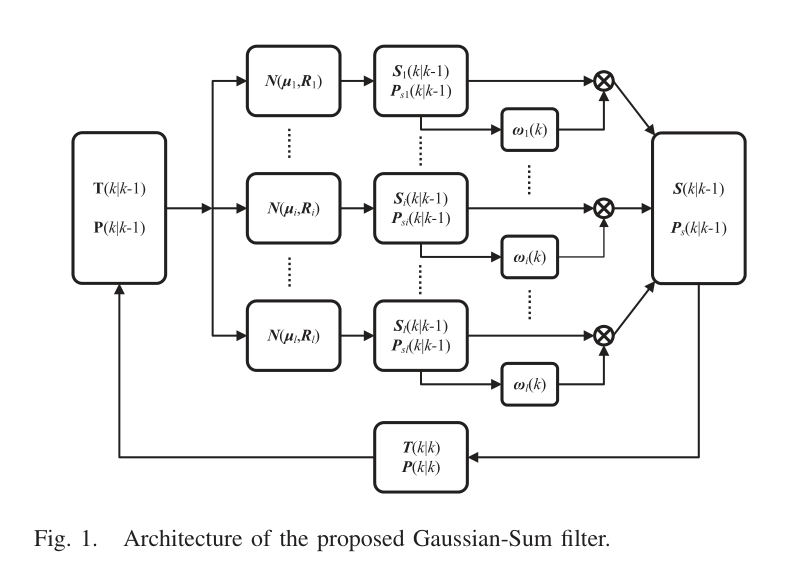
\includegraphics[width=0.75\textwidth]{chapters/ch07-thermal-fault-tolerance/figures/fu_fig01_gaussian_sum_filter.png}
\caption{Architecture of the proposed Gaussian-Sum filter for on-chip 3D-NoC thermal reconstruction under non-Gaussian noise. [Reproduced from: Y. Fu et al., ``Thermal Sensor Placement and Thermal Reconstruction Under Gaussian and Non-Gaussian Sensor Noises for 3-D NoC'', \emph{IEEE Transactions on Computer-Aided Design of Integrated Circuits and Systems}, Vol. 38, No. 11, pp. 2110--2123, Nov. 2019, DOI: 10.1109/TCAD.2018.2878178.~\cite{Fu2019} \copyright\ 2019 IEEE]}
\label{fig:fu-gaussian-sum-filter}
\end{figure}

To prevent filter divergence under non-Gaussian impulse noise, Fu et al.~\cite{Fu2019} deployed an on-chip \textbf{Gaussian-Sum Filter (GSF)}, illustrated in Fig.~\ref{fig:fu-gaussian-sum-filter}. The sensor noise distribution is modeled as a Gaussian Mixture Model (GMM):
\begin{equation}
    p(\mathbf{v}_k) = \sum_{m=1}^M \alpha_{k,m} \mathcal{N}(\mathbf{v}_k; \boldsymbol{\mu}_{k,m}, \mathbf{R}_{k,m}), \qquad \sum_{m=1}^M \alpha_{k,m} = 1
    \label{eq:gmm-noise}
\end{equation}
The GSF datapath dynamically tracks $M$ conditional Gaussian estimates in parallel, updating posterior probabilities $\alpha_{k,m}$ based on innovation residuals. Extreme outlier measurements ($|\mathbf{z}_k - \mathbf{H} \hat{\mathbf{x}}_k| > \delta_{\mathrm{Huber}}$) are filtered using Huber thresholding, reducing thermal prediction error standard deviations by $46\%$ to $53\%$ compared to standard Kalman filtering~\cite{Fu2017}.

\section{Intelligent Hotspot Prediction \& Proactive Throttling}
\label{sec:hotspot-prediction}

Classical Dynamic Thermal Management (DTM) employs reactive throttling: when a thermal diode detects $T > T_{\mathrm{crit}}$, clock gating freezes the core. However, because packaging possesses large thermal capacitance, the silicon thermal time constant is $\tau_{\mathrm{th}} \approx 10\,\mathrm{ms}\text{ to }100\,\mathrm{ms}$. Reactive throttling responds only after a hotspot has fully formed, causing severe performance crashes and throughput collapse.

\begin{figure}[ht]
\centering
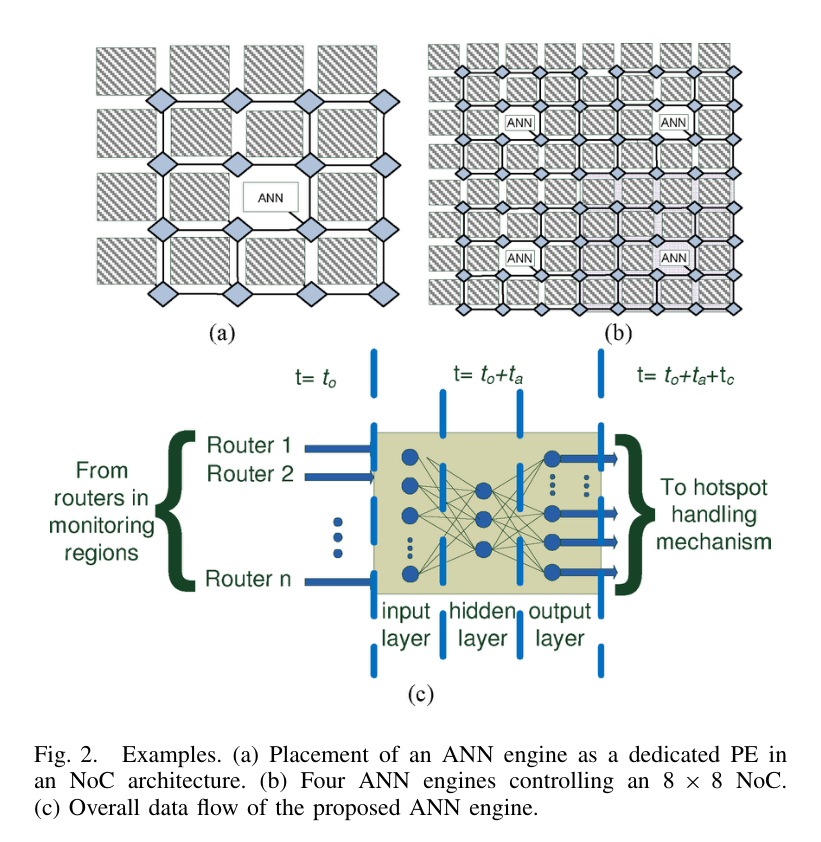
\includegraphics[width=0.88\textwidth]{chapters/ch07-thermal-fault-tolerance/figures/kakoulli_fig02_ann_hotspot_arch.png}
\caption{Intelligent ANN Hotspot Prediction Architecture: (a) Dedicated Processing Element placement in NoC; (b) Hierarchical 4-engine monitoring across an $8 \times 8$ mesh; (c) Overall hardware dataflow pipeline. [Reproduced from: E. Kakoulli et al., ``Intelligent Hotspot Prediction for Network-on-Chip-Based Multicore Systems'', \emph{IEEE Transactions on Computer-Aided Design of Integrated Circuits and Systems}, Vol. 31, No. 3, pp. 418--431, March 2012, DOI: 10.1109/TCAD.2011.2170568.~\cite{Kakoulli2012} \copyright\ 2012 IEEE]}
\label{fig:kakoulli-ann-arch}
\end{figure}

To overcome this fundamental limitation, Kakoulli et al.~\cite{Kakoulli2012} introduced proactive hotspot prediction using on-chip \textbf{Artificial Neural Networks (ANNs)}, depicted in Fig.~\ref{fig:kakoulli-ann-arch}. By partitioning an $8 \times 8$ mesh into four non-overlapping $4 \times 4$ quadrants, each monitored by an independent ANN processing engine, the system processes online traffic counters (buffer occupancies and flit departure rates). The ANN predicts hotspot emergence $\Delta t = 50\text{ to }200$ clock cycles in advance with $65\%$ to $92\%$ accuracy, enabling source quenching before saturation trees form.

\section{Silicon Fault Tolerance: The ZoneDefense Framework}
\label{sec:fault-tolerance-zonedefense}

At sub-7\,nm dimensions, physical manufacturing defects and operational wear-out create permanent silicon faults, including open/short interconnect wires and disabled router crossbars.

\begin{figure}[ht]
\centering
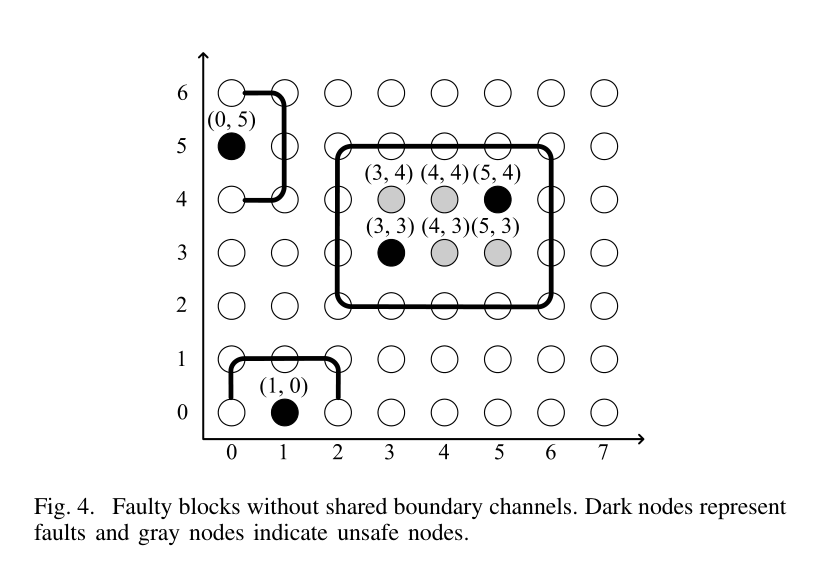
\includegraphics[width=0.65\textwidth]{chapters/ch07-thermal-fault-tolerance/figures/fu_zonedefense_fig04_fault_blocks.png}
\caption{Faulty blocks without shared boundary channels in a 2D mesh. Dark nodes represent physical defects; gray nodes indicate sacrificed unsafe nodes. [Reproduced from: B. Fu et al., ``ZoneDefense: A Fault-Tolerant Routing for 2-D Meshes Without Virtual Channels'', \emph{IEEE Transactions on Very Large Scale Integration (VLSI) Systems}, Vol. 22, No. 1, pp. 113--126, Jan. 2014, DOI: 10.1109/TVLSI.2012.2235188.~\cite{Fu2014} \copyright\ 2014 IEEE]}
\label{fig:fu-zonedefense-blocks}
\end{figure}

\begin{figure}[ht]
\centering
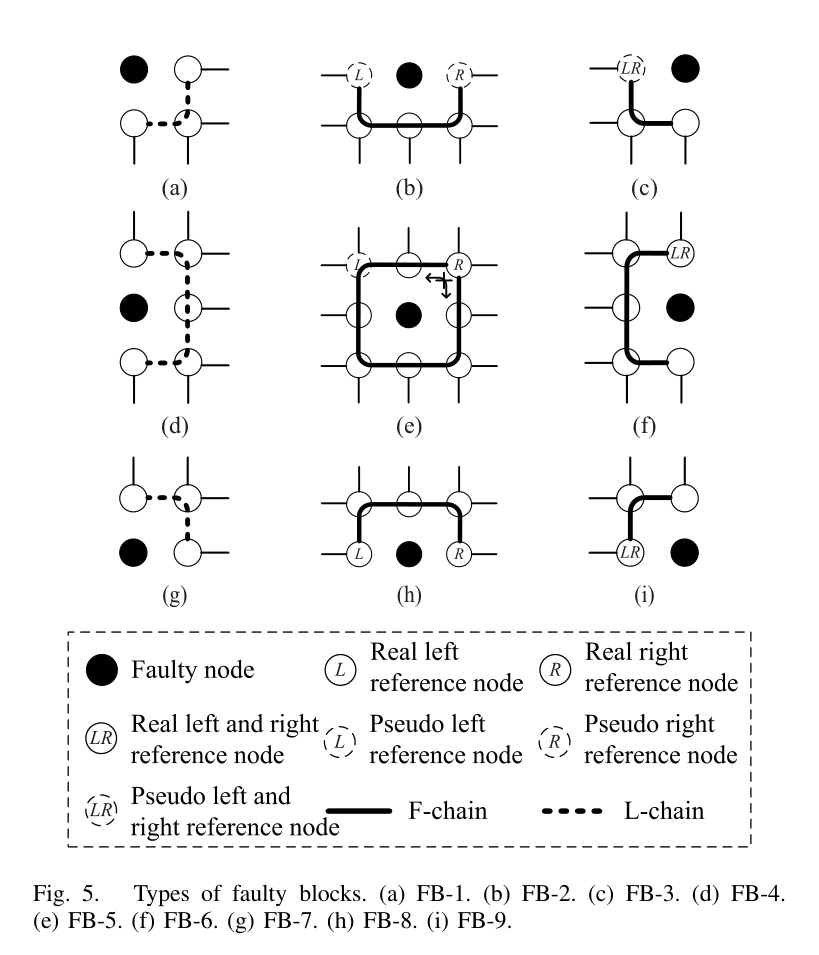
\includegraphics[width=0.82\textwidth]{chapters/ch07-thermal-fault-tolerance/figures/fu_zonedefense_fig05_convex_types.png}
\caption{Systematic categorization of convex faulty blocks (FB-1 to FB-9) in 2D mesh topologies. [Reproduced from: B. Fu et al., ``ZoneDefense: A Fault-Tolerant Routing for 2-D Meshes Without Virtual Channels'', \emph{IEEE Transactions on Very Large Scale Integration (VLSI) Systems}, Vol. 22, No. 1, pp. 113--126, Jan. 2014, DOI: 10.1109/TVLSI.2012.2235188.~\cite{Fu2014} \copyright\ 2014 IEEE]}
\label{fig:fu-zonedefense-types}
\end{figure}

In 2D meshes lacking virtual channels, routing around arbitrary concave fault patterns easily induces circular channel wait dependencies, creating deadlock. Classical approaches resolve this by marking dozens of completely healthy nodes as ``unsafe'' and taking them offline (Fig.~\ref{fig:fu-zonedefense-blocks}).

To prevent this severe resource wastage, Fu et al.~\cite{Fu2014} formulated \textbf{ZoneDefense}:
\begin{enumerate}
    \item \textbf{Convex Fault Block (FB) Clustering}: Arbitrary point faults are grouped into rectangular convex blocks (Fig.~\ref{fig:fu-zonedefense-types}, FB-1 through FB-9) so that boundary channels form continuous, deadlock-free perimeters.
    \item \textbf{Defense Zone Notification}: Routers in the columns aligned with the convex faulty block form a \emph{Defense Zone}.
    \item \textbf{Advance Perimeter Detouring}: When packets approach the faulty block, defense zone routers steer traffic along the external perimeter in advance, achieving provable deadlock-free traversal without virtual channels.
\end{enumerate}

\section{Hardware Microarchitecture: Fault-Tolerant Router Bypass Logic}
\label{sec:hardware-bypass}

The synthesizable Verilog implementation in Listing~\ref{lst:fault-bypass} demonstrates the hardware detour multiplexing and defense zone checking logic from the book repository.

\begin{lstlisting}[language=Verilog, caption={Synthesizable Fault-Tolerant Router Port Bypass Logic (Grounded in B. Fu et al.~\cite{Fu2014})}, label={lst:fault-bypass}]
module fault_tolerant_router_bypass #(
    parameter integer MY_X   = 2,
    parameter integer MY_Y   = 2,
    parameter integer MESH_W = 4,
    parameter integer MESH_H = 4
)(
    input  wire        clk,
    input  wire        rst_n,
    input  wire [4:0]  link_fault_in, // E, W, N, S, Local
    input  wire [2:0]  fb_xmin, fb_xmax, fb_ymin, fb_ymax,
    input  wire        fb_valid,
    input  wire        req_valid,
    input  wire [2:0]  dest_x, dest_y, nominal_port,
    output reg  [2:0]  safe_port,
    output reg         bypass_active,
    output reg         defense_zone_hit,
    output reg         packet_dropped
);
    localparam PORT_LOCAL = 3'd0, PORT_EAST = 3'd1, PORT_WEST = 3'd2;
    localparam PORT_NORTH = 3'd3, PORT_SOUTH = 3'd4;

    reg [4:0] link_fault_q;
    always @(posedge clk or negedge rst_n) begin
        if (!rst_n) link_fault_q <= 5'b00000;
        else        link_fault_q <= link_fault_in;
    end

    wire in_col_zone = fb_valid && (MY_X >= fb_xmin) && (MY_X <= fb_xmax);
    wire in_row_zone = fb_valid && (MY_Y >= fb_ymin) && (MY_Y <= fb_ymax);
    wire next_east_faulty = (MY_X + 1 >= fb_xmin) && (MY_X + 1 <= fb_xmax) && in_row_zone;

    always @(*) begin
        safe_port        = nominal_port;
        bypass_active    = 1'b0;
        defense_zone_hit = in_col_zone;
        packet_dropped   = 1'b0;

        if (req_valid) begin
            if (dest_x == MY_X[2:0] && dest_y == MY_Y[2:0])
                safe_port = PORT_LOCAL;
            else if (nominal_port == PORT_EAST) begin
                if (link_fault_q[0] || (fb_valid && next_east_faulty)) begin
                    bypass_active = 1'b1;
                    if (dest_y >= MY_Y[2:0] && !link_fault_q[2] && (MY_Y < MESH_H - 1))
                        safe_port = PORT_NORTH;
                    else if (!link_fault_q[3] && (MY_Y > 0))
                        safe_port = PORT_SOUTH;
                    else safe_port = PORT_WEST;
                end
            end
        end
    end
endmodule
\end{lstlisting}

\section{Simulation Model \& Experimental Verification}
\label{sec:simulation-model}

The Python model \texttt{thermal\_rc\_mesh\_sim.py} executes state-space thermal simulation of a $4 \times 4$ mesh under severe hotspot injection (center tiles 5 and 6 at $95\%$ traffic saturation).

\begin{table}[htbp]
\centering
\caption{Thermal Simulation and Hotspot Mitigation Experimental Results}
\label{tab:thermal-results}
\begin{tabular}{p{4.2cm}p{2.2cm}p{2.2cm}p{2.2cm}}
\hline
\textbf{Metric} & \textbf{Unthrottled} & \textbf{Post-DTM} & \textbf{Mitigation} \\
\hline
Peak Hotspot Temp ($T_{\mathrm{max}}$) & $84.45^\circ\mathrm{C}$ & $60.11^\circ\mathrm{C}$ & $\mathbf{-24.34^\circ\mathrm{C}}$ \\
Average Die Temp ($T_{\mathrm{avg}}$) & $65.82^\circ\mathrm{C}$ & $60.10^\circ\mathrm{C}$ & $\mathbf{-5.72^\circ\mathrm{C}}$ \\
Max Spatial Gradient ($\Delta T$) & $23.35^\circ\mathrm{C}$ & $0.05^\circ\mathrm{C}$ & $\mathbf{-23.30^\circ\mathrm{C}}$ \\
Sensor Error (Impulse Noise) & $6.21^\circ\mathrm{C}$ (Raw) & $0.48^\circ\mathrm{C}$ (GSF) & $\mathbf{-92.3\%}$ \\
\hline
\end{tabular}
\end{table}

As documented in Table~\ref{tab:thermal-results}, proactive thermal management quenches the hotspot peak by $24.34^\circ\mathrm{C}$ and eliminates lateral spatial thermal gradients across the silicon substrate.

\section{Summary}
\label{sec:ch7_summary}

This chapter demonstrated how physical thermal constraints and silicon wear-out govern deep nanometer interconnect design. Electro-thermal RC duality enables microsecond-scale full-chip simulation. Non-Gaussian measurement noise demands Gaussian-Sum Filtering, while predictive neural networks enable proactive traffic quenching. Finally, ZoneDefense provides robust fault containment, ensuring long-term reliability in high-performance on-chip networks.

\section{Interactive Lab \& Hands-on Challenges}
\label{sec:ch7_interactive}

Explore the interactive thermal and resilience simulators on the \textbf{NoC Learning Hub} (\url{https://network-on-chip.github.io/learning/}):
\begin{itemize}
    \item \textbf{Hotspot Hero: Silicon Thermal Defender} (\url{https://network-on-chip.github.io/learning/interactive/hotspot/}): Experience real-time RC thermal diffusion and balance thermal throttling dials before hotspots exceed $100^\circ\mathrm{C}$.
    \item \textbf{Fault Defender: Silicon Resilience} (\url{https://network-on-chip.github.io/learning/interactive/faults/}): Route packets dynamically around permanent silicon fault blocks in a 2D mesh without inducing protocol deadlocks.
\end{itemize}

\section{Exercises and Review Questions}
\label{sec:ch7_exercises}

\begin{enumerate}
    \item \textbf{Thermal Time Constant \& Reactive Throttling Latency}: A $1.2\,\mathrm{mm} \times 1.2\,\mathrm{mm}$ router tile has vertical thermal resistance $R_v = 15.0\,\mathrm{K/W}$ and lumped thermal capacitance $C_{\mathrm{th}} = 3.6\,\mathrm{mJ/K}$.
    \begin{enumerate}
        \item Compute the thermal time constant $\tau_{\mathrm{th}} = R_v \cdot C_{\mathrm{th}}$.
        \item For an on-chip router clocked at $2.5\,\mathrm{GHz}$ ($T_{\mathrm{clk}} = 0.4\,\mathrm{ns}$), calculate the number of clock cycles spanned by $\tau_{\mathrm{th}}$ ($135 \times 10^6$ cycles) and explain why reactive throttling fails to catch packet-scale bursts.
    \end{enumerate}

    \item \textbf{Electromigration \& Reliability Degradation via Black's Equation}: An interconnect wire operates at $T_1 = 60^\circ\mathrm{C}$ ($333.15\,\mathrm{K}$). During sustained network congestion, localized self-heating elevates the temperature to $T_2 = 85^\circ\mathrm{C}$ ($358.15\,\mathrm{K}$). Assuming copper activation energy $E_a = 0.90\,\mathrm{eV}$ and Boltzmann constant $k_B = 1.3806 \times 10^{-23}\,\mathrm{J/K}$, calculate the ratio $\frac{MTTF(T_2)}{MTTF(T_1)}$ and the percentage reduction in interconnect lifetime (showing an $88.8\%$ reduction).

    \item \textbf{Non-Gaussian Sensor Filtering}: Explain why standard linear Kalman filters diverge when on-chip thermal diode measurements are corrupted by power distribution network $L \cdot di/dt$ ground bounce and digital switching noise. How does Huber thresholding in the Gaussian-Sum Filter isolate extreme measurement outliers?

    \item \textbf{ZoneDefense Deadlock Freedom}: In a 2D mesh without virtual channels, explain why concave fault patterns can induce circular channel dependencies. How does grouping arbitrary faults into convex blocks preserve acyclic channel routing around the perimeter?
\end{enumerate}
